\chapterimage{chapter_head_2.pdf} % Chapter heading image

\chapter{Funções e operadores notáveis}

%%%%%%%%%%%%%%%%%%%%%%%%%%%%%%%%%%%%%%%%%%%%%%%%%%%%%%%%%%%%%%%%%%%%%%%%%%%%%%%%%%%%%%%
%%%%%%%%%%%%%%%%%%%%%%%%%%%%%%%%%%%%%%%%%%%%%%%%%%%%%%%%%%%%%%%%%%%%%%%%%%%%%%%%%%%%%%%
%%%%%%%%%%%%%%%%%%%%%%%%%%%%%%%%%%%%%%%%%%%%%%%%%%%%%%%%%%%%%%%%%%%%%%%%%%%%%%%%%%%%%%%
\section{Operador derivada para $e(\VECTOR{x})$, $\VECTOR{f}(\VECTOR{x})$ e  $\MATRIX{G}(\VECTOR{x})$}

\begin{definition}\label{def:deltahor}
Se 
$\VECTOR{x}\in \mathbb{R}^N$ é um vetor coluna com elementos $x_n\in \mathbb{R}$ de modo que
$n\in \mathbb{N}$, $1 \leq n \leq N$, 
a função $e(\VECTOR{x}): \mathbb{R}^N \rightarrow \mathbb{R}$ é um escalar, 
a função $\VECTOR{f}(\VECTOR{x}): \mathbb{R}^N \rightarrow \mathbb{R}^M$ é um vetor coluna,  e
a função $\MATRIX{G}(\VECTOR{x}): \mathbb{R}^N \rightarrow \mathbb{R}^{M\times L}$ é uma matriz, 
então definimos que:

\begin{equation}
\frac{\partial e(\VECTOR{x}) }{\partial \VECTOR{x}^{\transpose}}= 
\left[
\begin{matrix}
\frac{\partial e(\VECTOR{x}) }{\partial x_{1}}&
\frac{\partial e(\VECTOR{x}) }{\partial x_{2}}&
\hdots&
\frac{\partial e(\VECTOR{x}) }{\partial x_{n}}&
\hdots&
\frac{\partial e(\VECTOR{x}) }{\partial x_{N}}
\end{matrix}
\right]= {\bigcup\limits_{n=1}^{\rightarrow}}^{N}{\frac{\partial e(\VECTOR{x}) }{\partial x_{n}}} 
\end{equation}

\begin{equation}
\frac{\partial \VECTOR{f}(\VECTOR{x}) }{\partial \VECTOR{x}^{\transpose}}= 
\left[
\begin{matrix}
\frac{\partial \VECTOR{f}(\VECTOR{x}) }{\partial x_{1}}&
\frac{\partial \VECTOR{f}(\VECTOR{x}) }{\partial x_{2}}&
\hdots&
\frac{\partial \VECTOR{f}(\VECTOR{x}) }{\partial x_{n}}&
\hdots&
\frac{\partial \VECTOR{f}(\VECTOR{x}) }{\partial x_{N}}
\end{matrix}
\right]= {\bigcup\limits_{n=1}^{\rightarrow}}^{N}{\frac{\partial \VECTOR{f}(\VECTOR{x}) }{\partial x_{n}}} 
\end{equation}

\begin{equation}
\frac{\partial \MATRIX{G}(\VECTOR{x}) }{\partial \VECTOR{x}^{\transpose}}= 
\left[
\begin{matrix}
\frac{\partial \MATRIX{G}(\VECTOR{x}) }{\partial x_{1}}&
\frac{\partial \MATRIX{G}(\VECTOR{x}) }{\partial x_{2}}&
\hdots&
\frac{\partial \MATRIX{G}(\VECTOR{x}) }{\partial x_{n}}&
\hdots&
\frac{\partial \MATRIX{G}(\VECTOR{x}) }{\partial x_{N}}
\end{matrix}
\right]= {\bigcup\limits_{n=1}^{\rightarrow}}^{N}{\frac{\partial \MATRIX{G}(\VECTOR{x}) }{\partial x_{n}}}.
\end{equation}

Assim, 
$\frac{\partial e(\VECTOR{x}) }{\partial \VECTOR{x}^{\transpose}} \in \mathbb{R}^{1\times N}$,
$\frac{\partial \VECTOR{f}(\VECTOR{x}) }{\partial \VECTOR{x}^{\transpose}} \in \mathbb{R}^{M \times N}$ e
$\frac{\partial \VECTOR{g}(\VECTOR{x}) }{\partial \VECTOR{x}^{\transpose}} \in \mathbb{R}^{M \times (LN)}$.
\end{definition}

\begin{definition}\label{def:deltaver}
Se 
$\VECTOR{x}\in \mathbb{R}^N$ é um vetor coluna com elementos $x_n\in \mathbb{R}$ de modo que
$n\in \mathbb{N}$, $1 \leq n \leq N$, 
a função $e(\VECTOR{x}): \mathbb{R}^N \rightarrow \mathbb{R}$ é um escalar,
a função $\VECTOR{f}(\VECTOR{x}): \mathbb{R}^N \rightarrow \mathbb{R}^M$ é um vetor coluna,  e
a função $\MATRIX{G}(\VECTOR{x}): \mathbb{R}^N \rightarrow \mathbb{R}^{M\times L}$ é uma matriz, 
então definimos que:
\begin{equation}
\frac{\partial e(\VECTOR{x}) }{\partial \VECTOR{x}}= 
\left[
\begin{matrix}
\frac{\partial e(\VECTOR{x}) }{\partial x_{1}} \\
\frac{\partial e(\VECTOR{x}) }{\partial x_{2}} \\
\vdots \\
\frac{\partial e(\VECTOR{x}) }{\partial x_{n}} \\
\vdots \\
\frac{\partial e(\VECTOR{x}) }{\partial x_{N}} 
\end{matrix}
\right] = \functrans \left( \frac{\partial e(\VECTOR{x}) }{\partial \VECTOR{x}^{\transpose}} \right) =
\funcvec \left( \frac{\partial e(\VECTOR{x}) }{\partial \VECTOR{x}^{\transpose}} \right) =
{\bigcup\limits_{n=1}^{\downarrow}}^{N}{\frac{\partial e(\VECTOR{x}) }{\partial x_{n}}} 
\end{equation}

\begin{equation}
\frac{\partial \VECTOR{f}(\VECTOR{x}) }{\partial \VECTOR{x}}= 
\left[
\begin{matrix}
\frac{\partial \VECTOR{f}(\VECTOR{x}) }{\partial x_{1}} \\
\frac{\partial \VECTOR{f}(\VECTOR{x}) }{\partial x_{2}} \\
\vdots \\
\frac{\partial \VECTOR{f}(\VECTOR{x}) }{\partial x_{n}} \\
\vdots \\
\frac{\partial \VECTOR{f}(\VECTOR{x}) }{\partial x_{N}}
\end{matrix}
\right] =  \funcvec \left( \frac{\partial \VECTOR{f}(\VECTOR{x}) }{\partial \VECTOR{x}^{\transpose}} \right) =
{\bigcup\limits_{n=1}^{\downarrow}}^{N}{\frac{\partial \VECTOR{f}(\VECTOR{x}) }{\partial x_{n}}}
\end{equation}

\begin{equation}
\frac{\partial \MATRIX{G}(\VECTOR{x}) }{\partial \VECTOR{x}}= 
\left[
\begin{matrix}
\frac{\partial \MATRIX{G}(\VECTOR{x}) }{\partial x_{1}} \\
\frac{\partial \MATRIX{G}(\VECTOR{x}) }{\partial x_{2}} \\
\vdots \\
\frac{\partial \MATRIX{G}(\VECTOR{x}) }{\partial x_{n}} \\
\vdots \\
\frac{\partial \MATRIX{G}(\VECTOR{x}) }{\partial x_{N}}
\end{matrix}
\right] = {\bigcup\limits_{n=1}^{\downarrow}}^{N}{\frac{\partial \MATRIX{G}(\VECTOR{x}) }{\partial x_{n}}}
\end{equation}

Assim, 
$\frac{\partial e(\VECTOR{x}) }{\partial \VECTOR{x}} \in \mathbb{R}^{N \times 1}$,
$\frac{\partial \VECTOR{f}(\VECTOR{x}) }{\partial \VECTOR{x}} \in \mathbb{R}^{(MN) \times 1}$ e
$\frac{\partial \VECTOR{g}(\VECTOR{x}) }{\partial \VECTOR{x}} \in \mathbb{R}^{(MN) \times L}$.
\end{definition}


\begin{corollary}[Igualdade das derivadas cruzadas]\label{cor:derder}
Se 
$\VECTOR{x}\in \mathbb{R}^N$ é um vetor coluna com elementos $x_n\in \mathbb{R}$ de modo que
$n\in \mathbb{N}$, $1 \leq n \leq N$, 
a função $e(\VECTOR{x}): \mathbb{R}^N \rightarrow \mathbb{R}$ é um escalar,
e tendo em consideração as Definições \ref{def:deltahor} e \ref {def:deltaver} e o 
``Teorema da igualdade das derivadas cruzadas'' \FALTAREFERENCIA; então é fácil deduzir que:
\begin{equation}
 \frac{\partial }{\partial \VECTOR{x}} \left( \frac{\partial e(\VECTOR{x} )}{\partial \VECTOR{x}^{\transpose}} \right) \equiv \frac{\partial }{\partial \VECTOR{x}^{\transpose}} \left( \frac{\partial e(\VECTOR{x} )}{\partial \VECTOR{x}} \right)
\end{equation}
\end{corollary}

%%%%%%%%%%%%%%%%%%%%%%%%%%%%%%%%%%%%%%%%%%%%%%%%%%%%%%%%%%%%%%%%%%%%%%%%%%%%%%%%%%%%%%%
%%%%%%%%%%%%%%%%%%%%%%%%%%%%%%%%%%%%%%%%%%%%%%%%%%%%%%%%%%%%%%%%%%%%%%%%%%%%%%%%%%%%%%%
%%%%%%%%%%%%%%%%%%%%%%%%%%%%%%%%%%%%%%%%%%%%%%%%%%%%%%%%%%%%%%%%%%%%%%%%%%%%%%%%%%%%%%%
\section{Derivadas notáveis: Gradiente, Matriz Hessiana, Matriz Jacobiana}

\begin{proposition}[Gradiente de $e(\VECTOR{x})$]\label{def:gradient}
 Dada uma função $e:\mathbb{R}^{N}\rightarrow \mathbb{R}$ com variável $\VECTOR{x} \in \mathbb{R}^{N}$
 como vetor coluna com elementos $x_n\in \mathbb{R}$ de modo que $n\in \mathbb{N}$, $1 \leq n \leq N$,
 diferenciável em $\VECTOR{x}$. 
 $\triangledown e(\VECTOR{x})$ é chamado gradiente \cite{Gradient} \FALTAREFERENCIA   de $e(\VECTOR{x})$, de modo que: 
 \begin{equation}
  \triangledown e(\VECTOR{x})\equiv \frac{\partial e(\VECTOR{x})}{\partial \VECTOR{x}^{\transpose} }=
\left[
\begin{matrix}
\frac{\partial e(\VECTOR{x}) }{\partial x_{1}}&
\frac{\partial e(\VECTOR{x}) }{\partial x_{2}}&
\hdots&
\frac{\partial e(\VECTOR{x}) }{\partial x_{n}}&
\hdots&
\frac{\partial e(\VECTOR{x}) }{\partial x_{N}}
\end{matrix}
\right]
 \end{equation}
\end{proposition}
\index{Gradiente}


\begin{proposition}[Matriz Hessiana de $e(\VECTOR{x})$]\label{def:hessian}
 Dada uma função $e:\mathbb{R}^{N}\rightarrow \mathbb{R}$ com variável $\VECTOR{x} \in \mathbb{R}^{N}$
 como vetor coluna  com elementos $x_n\in \mathbb{R}$ de modo que $n\in \mathbb{N}$, $1 \leq n \leq N$,
 diferenciável em $\VECTOR{x}$. 
 $\MATRIX{H}(\VECTOR{x})$ é chamada matriz Hessiana \cite{Hessian} \FALTAREFERENCIA   de $e(\VECTOR{x})$, de modo que: 
 \begin{equation}
  \MATRIX{H}(\VECTOR{x})\equiv \frac{\partial }{\partial \VECTOR{x}} \left( \frac{\partial e(\VECTOR{x})}{ \partial \VECTOR{x}^{\transpose} }\right)=
\left[
\begin{matrix}
\frac{\partial^2 e(\VECTOR{x}) }{\partial x_{1}\partial x_{1}}&
\frac{\partial^2 e(\VECTOR{x}) }{\partial x_{1}\partial x_{2}}&
\hdots&
\frac{\partial^2 e(\VECTOR{x}) }{\partial x_{1}\partial x_{n}}&
\hdots&
\frac{\partial^2 e(\VECTOR{x}) }{\partial x_{1}\partial x_{N}}\\
\frac{\partial^2 e(\VECTOR{x}) }{\partial x_{2}\partial x_{1}}&
\frac{\partial^2 e(\VECTOR{x}) }{\partial x_{2}\partial x_{2}}&
\hdots&
\frac{\partial^2 e(\VECTOR{x}) }{\partial x_{2}\partial x_{n}}&
\hdots&
\frac{\partial^2 e(\VECTOR{x}) }{\partial x_{2}\partial x_{N}}\\
\vdots&
\vdots&
\vdots&
\vdots&
\vdots&
\vdots\\
\frac{\partial^2 e(\VECTOR{x}) }{\partial x_{m}\partial x_{1}}&
\frac{\partial^2 e(\VECTOR{x}) }{\partial x_{m}\partial x_{2}}&
\hdots&
\frac{\partial^2 e(\VECTOR{x}) }{\partial x_{m}\partial x_{n}}&
\hdots&
\frac{\partial^2 e(\VECTOR{x}) }{\partial x_{m}\partial x_{N}}\\
\vdots&
\vdots&
\vdots&
\vdots&
\vdots&
\vdots\\
\frac{\partial^2 e(\VECTOR{x}) }{\partial x_{M}\partial x_{1}}&
\frac{\partial^2 e(\VECTOR{x}) }{\partial x_{M}\partial x_{2}}&
\hdots&
\frac{\partial^2 e(\VECTOR{x}) }{\partial x_{M}\partial x_{n}}&
\hdots&
\frac{\partial^2 e(\VECTOR{x}) }{\partial x_{M}\partial x_{N}}\\
\end{matrix}
\right]
 \end{equation}
\end{proposition}
\index{Matriz Hessiana}

\begin{proposition}[Matriz Jacobiana de $\VECTOR{f}(\VECTOR{x})$]\label{def:jacobian}
 Dado um vetor coluna, como função $\VECTOR{f}:\mathbb{R}^{N}\rightarrow \mathbb{R}^{M}$ com variável $\VECTOR{x} \in \mathbb{R}^{N}$
 como vetor coluna com elementos $x_n\in \mathbb{R}$ de modo que $n\in \mathbb{N}$, $1 \leq n \leq N$,
 diferenciável em $\VECTOR{x}$. 
 $\MATRIX{J}(\VECTOR{x})$ é chamada matriz Jacobiana \cite{Jacobian} \FALTAREFERENCIA   de 
 $\VECTOR{f}(\VECTOR{x})=[f_1(\VECTOR{x})~f_2(\VECTOR{x})~\dots~f_m(\VECTOR{x})~\dots f_M(\VECTOR{x})]^{\transpose}$, de modo que: 
 \begin{equation}
  \MATRIX{J}(\VECTOR{x})\equiv \frac{\partial \VECTOR{f}(\VECTOR{x})}{\partial \VECTOR{x}^{\transpose} }=
\left[
\begin{matrix}
\frac{\partial \VECTOR{f}(\VECTOR{x}) }{\partial x_{1}}&
\frac{\partial \VECTOR{f}(\VECTOR{x}) }{\partial x_{2}}&
\hdots&
\frac{\partial \VECTOR{f}(\VECTOR{x}) }{\partial x_{n}}&
\hdots&
\frac{\partial \VECTOR{f}(\VECTOR{x}) }{\partial x_{N}}
\end{matrix}
\right]
 \end{equation}
  \begin{equation}
  \MATRIX{J}(\VECTOR{x})\equiv 
\left[
\begin{matrix}
\frac{\partial f_1(\VECTOR{x}) }{\partial x_{1}}&
\frac{\partial f_1(\VECTOR{x}) }{\partial x_{2}}&
\hdots&
\frac{\partial f_1(\VECTOR{x}) }{\partial x_{n}}&
\hdots&
\frac{\partial f_1(\VECTOR{x}) }{\partial x_{N}}\\
\frac{\partial f_2(\VECTOR{x}) }{\partial x_{1}}&
\frac{\partial f_2(\VECTOR{x}) }{\partial x_{2}}&
\hdots&
\frac{\partial f_2(\VECTOR{x}) }{\partial x_{n}}&
\hdots&
\frac{\partial f_2(\VECTOR{x}) }{\partial x_{N}}\\
\vdots&
\vdots&
\hdots&
\vdots&
\vdots&
\vdots\\
\frac{\partial f_m(\VECTOR{x}) }{\partial x_{1}}&
\frac{\partial f_m(\VECTOR{x}) }{\partial x_{2}}&
\hdots&
\frac{\partial f_m(\VECTOR{x}) }{\partial x_{n}}&
\hdots&
\frac{\partial f_m(\VECTOR{x}) }{\partial x_{N}}\\
\vdots&
\vdots&
\hdots&
\vdots&
\vdots&
\vdots\\
\frac{\partial f_M(\VECTOR{x}) }{\partial x_{1}}&
\frac{\partial f_M(\VECTOR{x}) }{\partial x_{2}}&
\hdots&
\frac{\partial f_M(\VECTOR{x}) }{\partial x_{n}}&
\hdots&
\frac{\partial f_M(\VECTOR{x}) }{\partial x_{N}}\\
\end{matrix}
\right]
 \end{equation}
\end{proposition}
\index{Matriz Jacobiana}

%%%%%%%%%%%%%%%%%%%%%%%%%%%%%%%%%%%%%%%%%%%%%%%%%%%%%%%%%%%%%%%%%%%%%%%%%%%%%%%%%%%%%%%
%%%%%%%%%%%%%%%%%%%%%%%%%%%%%%%%%%%%%%%%%%%%%%%%%%%%%%%%%%%%%%%%%%%%%%%%%%%%%%%%%%%%%%%
%%%%%%%%%%%%%%%%%%%%%%%%%%%%%%%%%%%%%%%%%%%%%%%%%%%%%%%%%%%%%%%%%%%%%%%%%%%%%%%%%%%%%%%
\section{Serie de Taylor de $d(x)$, $e(\VECTOR{x})$ e $\VECTOR{f}(\VECTOR{x})$}
\label{def:taylor}
\index{Serie de Taylor}

\begin{proposition}[Serie de Taylor de $d(x)$]\label{prop:taylord}
Dada uma função $d:\mathbb{R}\rightarrow \mathbb{R}$ com variável $x \in \mathbb{R}$;
infinitamente diferenciável em $a \in \mathbb{R}$;
esta pode ser expressada mediante uma somatória, em serie de Taylor \cite{Taylor} \FALTAREFERENCIA ao redor de $a$, como
mostra a Eq. (\ref{eq:taylord1}),
\begin{equation}\label{eq:taylord1}
  d(x)=d(a)
      ~+\left.\frac{\partial   d(x)}{\partial x  }\right|_{x=a}(x-a)
      ~+\frac{1}{2}\left.\frac{\partial^2 d(x)}{\partial x^2}\right|_{x=a}(x-a)^{2}
      ~+\cdots 
      ~+\frac{1}{k!}\left.\frac{\partial^k d(x)}{\partial x^k}\right|_{x=a}(x-a)^{k}
      ~+\cdots 
\end{equation}
A equação pode ser escrita de forma mais compacta mediante uma somatória  como mostra a Eq. (\ref{eq:taylord2}),
\begin{equation}\label{eq:taylord2}
  d(x)=\sum\limits_{k=0}^{+\infty} \left.\frac{\partial^k d(x)}{\partial x^k}\right|_{x=a}\frac{(x-a)^{k}}{k!}.
\end{equation}
\end{proposition}

É possível ver um exemplo de aproximação da função $cos(x)$, 
mediante o uso da serie de Taylor da Proposição \ref{prop:taylord}, 
truncada ate a derivada de ordem $4$, $8$ e $10$, na Fig. \ref{fig:taylore}.
\begin{figure}[!h]
  \centering
    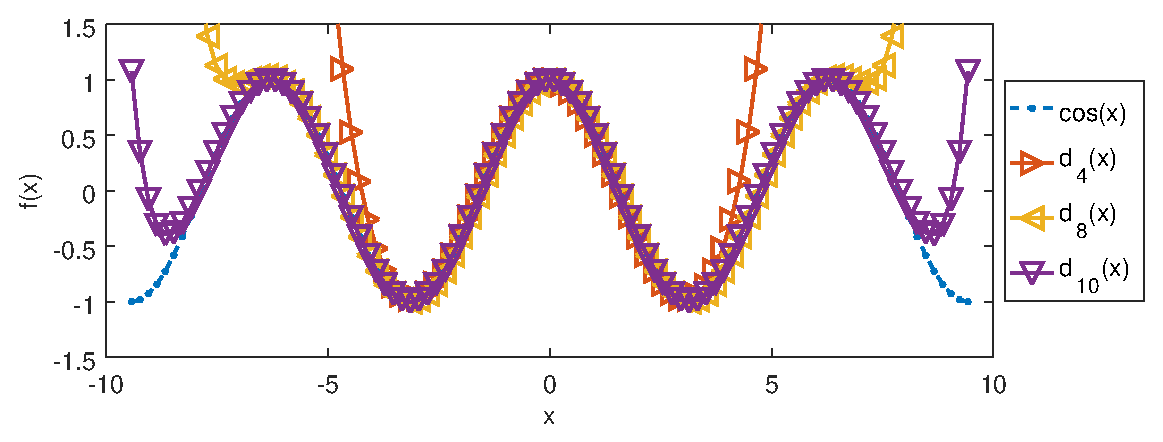
\includegraphics[width=0.8\textwidth]{chapters/funcoes/mcode/taylore.eps}
  \caption{Aproximação da função $cos(x)$ usando a serie de Taylor truncada.}
    \label{fig:taylore}
\end{figure}
 
 
\begin{proposition}[Serie de Taylor de $e(\VECTOR{x})$]\label{prop:taylore}
Dada uma função $e:\mathbb{R}^{N}\rightarrow \mathbb{R}$ com variável $\VECTOR{x} \in \mathbb{R}^{N}$, vetor coluna;
infinitamente diferenciável em $\VECTOR{a} \in \mathbb{R}^{N}$;
esta pode ser expressada mediante uma somatória, em serie de Taylor \cite{Taylor} \FALTAREFERENCIA ao redor de $\VECTOR{a}$, como
mostra a Eq. (\ref{eq:taylore1}),
\begin{equation}\label{eq:taylore1}
e(\VECTOR{x}) =\sum _{k_{1}=0}^{\infty }\cdots \sum _{k_{N}=0}^{\infty }\left.\left({\frac {\partial ^{k_{1}+\cdots +k_{N}}e(\VECTOR{x})}{\partial x_{1}^{k_{1}}\cdots \partial x_{N}^{k_{N}}}}\right)\right|_{\VECTOR{x}=\VECTOR{a}} {\frac {(x_{1}-a_{1})^{k_{1}}\cdots (x_{N}-a_{N})^{k_{N}}}{k_{1}!\cdots k_{N}!}}
\end{equation}

Outra forma alternativa de expressar a função anterior é usando vetores e matrizes,
como na Eq. (\ref{eq:taylore2}).
\begin{equation}\label{eq:taylore2}
  e(\VECTOR{x})=e(\VECTOR{a})
      ~+ \triangledown e(\VECTOR{a}) (\VECTOR{x}-\VECTOR{a})
      ~+\frac{1}{2!}(\VECTOR{x}-\VECTOR{a})^{\transpose} \MATRIX{H(\VECTOR{a})}  (\VECTOR{x}-\VECTOR{a})
      ~+\cdots 
\end{equation}
Onde o vector $\triangledown e(\VECTOR{x})\equiv \frac{\partial e(\VECTOR{x})}{\partial \VECTOR{x}^{\transpose} }$ 
(também chamado \hyperref[def:gradient]{gradiente}),
e a matriz $\MATRIX{H}(\VECTOR{x})\equiv \frac{\partial }{\partial \VECTOR{x}} \left( \frac{\partial e(\VECTOR{x})}{ \partial \VECTOR{x}^{\transpose} }\right)$
(também chamada matriz \hyperref[def:hessian]{Hessiana}).
\end{proposition}
\index{Matriz Hessiana}
\index{Gradiente}

\begin{proposition}[Serie de Taylor de $\VECTOR{f}(\VECTOR{x})$]\label{prop:taylorf}
Dada uma função de contra-domino vectorial $\VECTOR{f}:\mathbb{R}^{N}\rightarrow \mathbb{R}^{M}$, 
sendo $\VECTOR{f}$ um vector coluna, com variável $\VECTOR{x} \in \mathbb{R}^{N}$, vetor coluna;
infinitamente diferenciável em $\VECTOR{a} \in \mathbb{R}^{N}$;
esta pode ser expressada mediante uma somatória, em serie de Taylor \cite{Taylor} \FALTAREFERENCIA ao redor de $\VECTOR{a}$, como
mostra a Eq. (\ref{eq:taylorf1}),
\begin{equation}\label{eq:taylorf1}
\VECTOR{f}(\VECTOR{x}) =\VECTOR{f}(\VECTOR{a})
      ~+ \MATRIX{J}(\VECTOR{a}) (\VECTOR{x}-\VECTOR{a})
      ~+\cdots 
\end{equation}

Onde a matriz $\MATRIX{J}(\VECTOR{x})\equiv \frac{\partial \VECTOR{f}(\VECTOR{x})}{\partial \VECTOR{x}^{\transpose} }$,
também conhecido como matriz \hyperref[def:jacobian]{Jacobiana} de $\VECTOR{f}(\VECTOR{x})$.
\end{proposition}
\index{Matriz Jacobiana}